\documentclass[12pt,prb,aps,epsf]{article}
\usepackage[utf8]{inputenc}
\usepackage{amsmath}
\usepackage{amsfonts}
\usepackage{amssymb}
\usepackage{graphicx} 
\usepackage{latexsym} 
\usepackage[toc,page]{appendix}
%\usepackage{listings}
\usepackage{xcolor}
\usepackage{soul}
\usepackage[T1]{fontenc}
\usepackage{amsthm}
\usepackage{mathtools}
\usepackage{setspace}
\usepackage{array,multirow,makecell}
\usepackage{geometry}
\usepackage{textcomp}
\usepackage{float}
\usepackage{cancel}
\usepackage{here}
\usepackage{titlesec}
\usepackage{bbold}

\geometry{hmargin=2cm,vmargin=2cm}

\begin{document}
	
	\title{MP 21 Production et conversion d'énergie électrique}
	\author{Etienne}
	\date{Agrégation 2019}
	
	\maketitle
	
	\tableofcontents
	
	\pagebreak
	
\subsection{Introduction}
La production d'énergie est cruciale : donner la production et la consommation annuelle ou journalière française.. Il existe différents moyens de la produire..
\section{Production : le panneau photovoltaïque}
\begin{figure}
	\centering 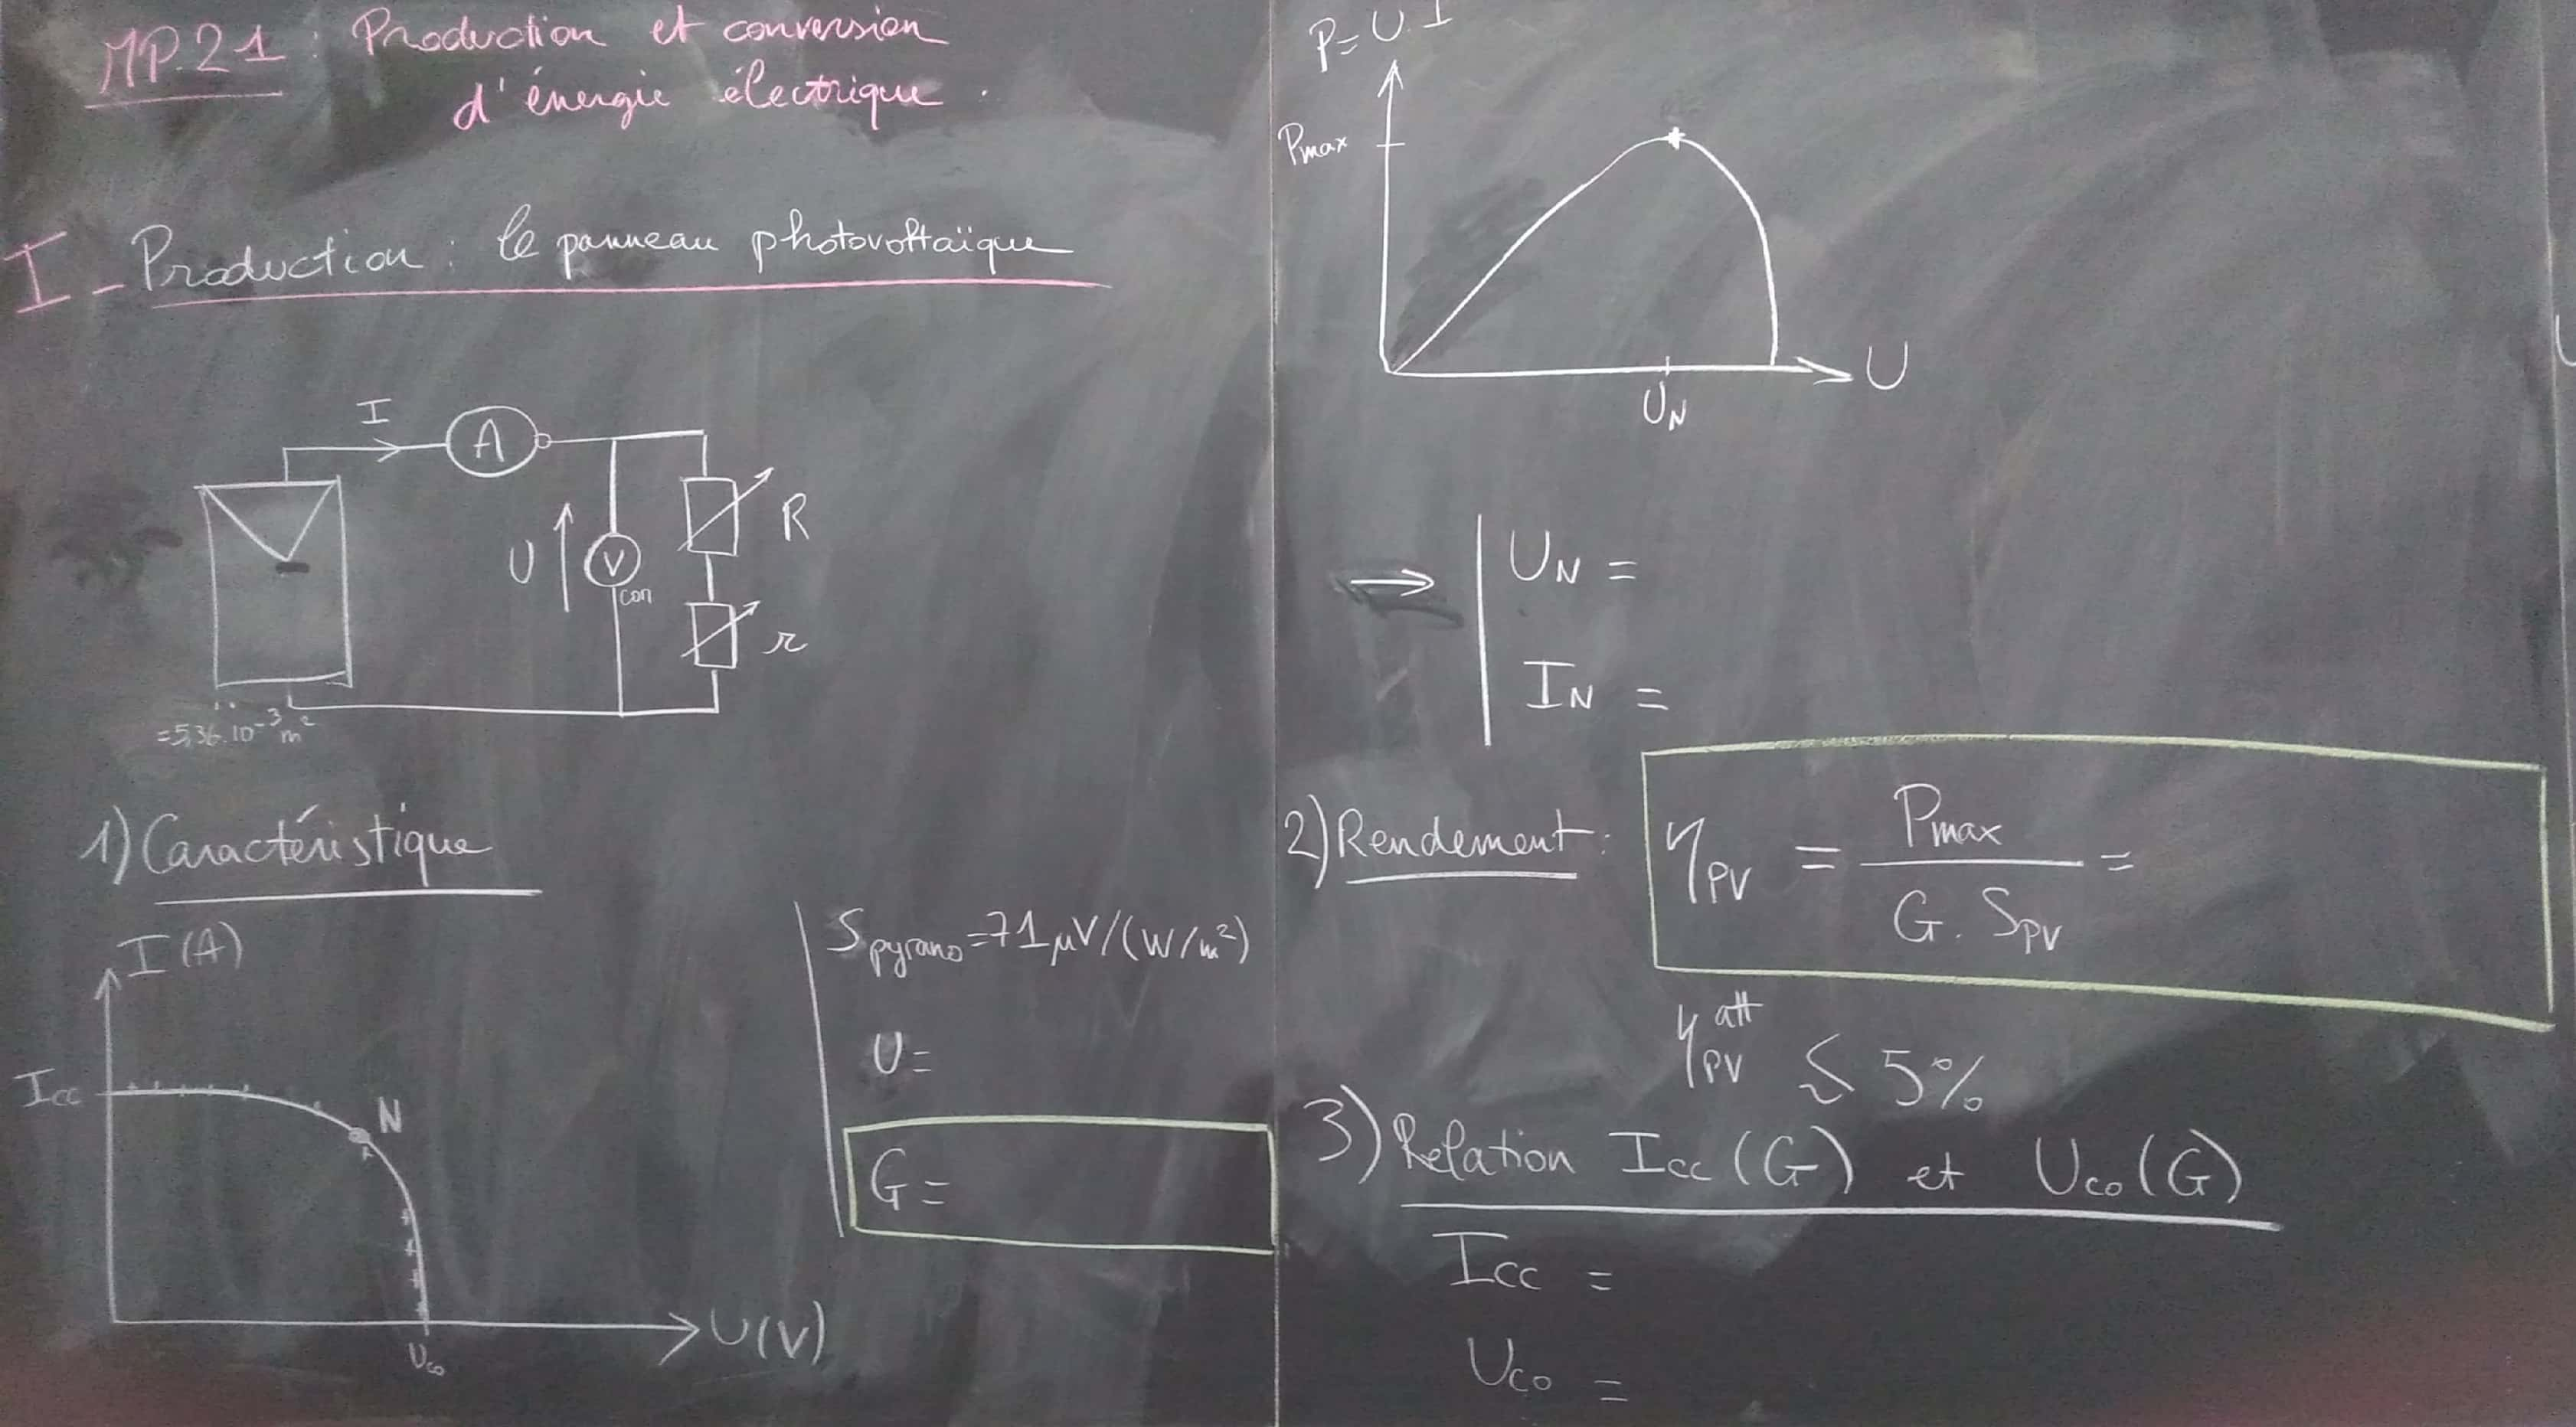
\includegraphics[width=18cm]{T1}
\end{figure}

\subsection{Caractéristique}
On mesure la valeur de l'irradiance produite par la lampe (puissance lumineuse surfacique en $W.m^{-2}$) au pyranomètre. On place ensuite notre panneau photovoltaïque sous cette lampe, on le relie à une résistance réglable et on trace alors la caractéristique en mesurant $I$ et $U$ tout en faisant varier à chaque fois la résistance. Afin d'avoir une courbe esthétique on commence par faire varier $U$ de manière régulière, puis fait ensuite varier l'intensité $I$ de manière régulière lorsqu'on a passé le point nominal.\\

On peut estimer la tension nominale en traçant 
\begin{eqnarray}
P = U\,I = f(U)
\end{eqnarray}

\subsection{Rendement}
Une fois le point de fonctionnement nominal identifié, on peut calculer le rendement 
\begin{eqnarray}
\eta_{PV} = \frac{P_{max}}{G\,S_{PV}} = 3,8\,\%
\end{eqnarray}
avec $G$ l'irradiance et $S_{PV}$ la surface du panneau, a comparer avec les infos constructeur qui nous l'annonce à 5\%.

\subsection{Relation Icc(G) et Uco(G)}
On note $Icc$ le courant de court circuit et $Uco$ la tension en circuit ouvert.\\

On remarque en notant les valeurs de $Icc$, $Uco$ pour différentes valeur de l'irradiance $G$ que l'on a 
\begin{eqnarray}
Icc \propto G\\
Uco \;\mathrm{independant\;de}\; G
\end{eqnarray}

Lorsque l'irradiance varie (nuage, poussière...) la résistance en sortie du panneau elle ne varie pas, et on se retrouve alors à un point de fonctionnement non optimal. Il faut donc faire varier la tension de sortie pour se replacer au point nominal de la caractéristique du panneau, ce que l'on peut faire à l'aide d'un hacheur.

\begin{figure}[h]
	\centering 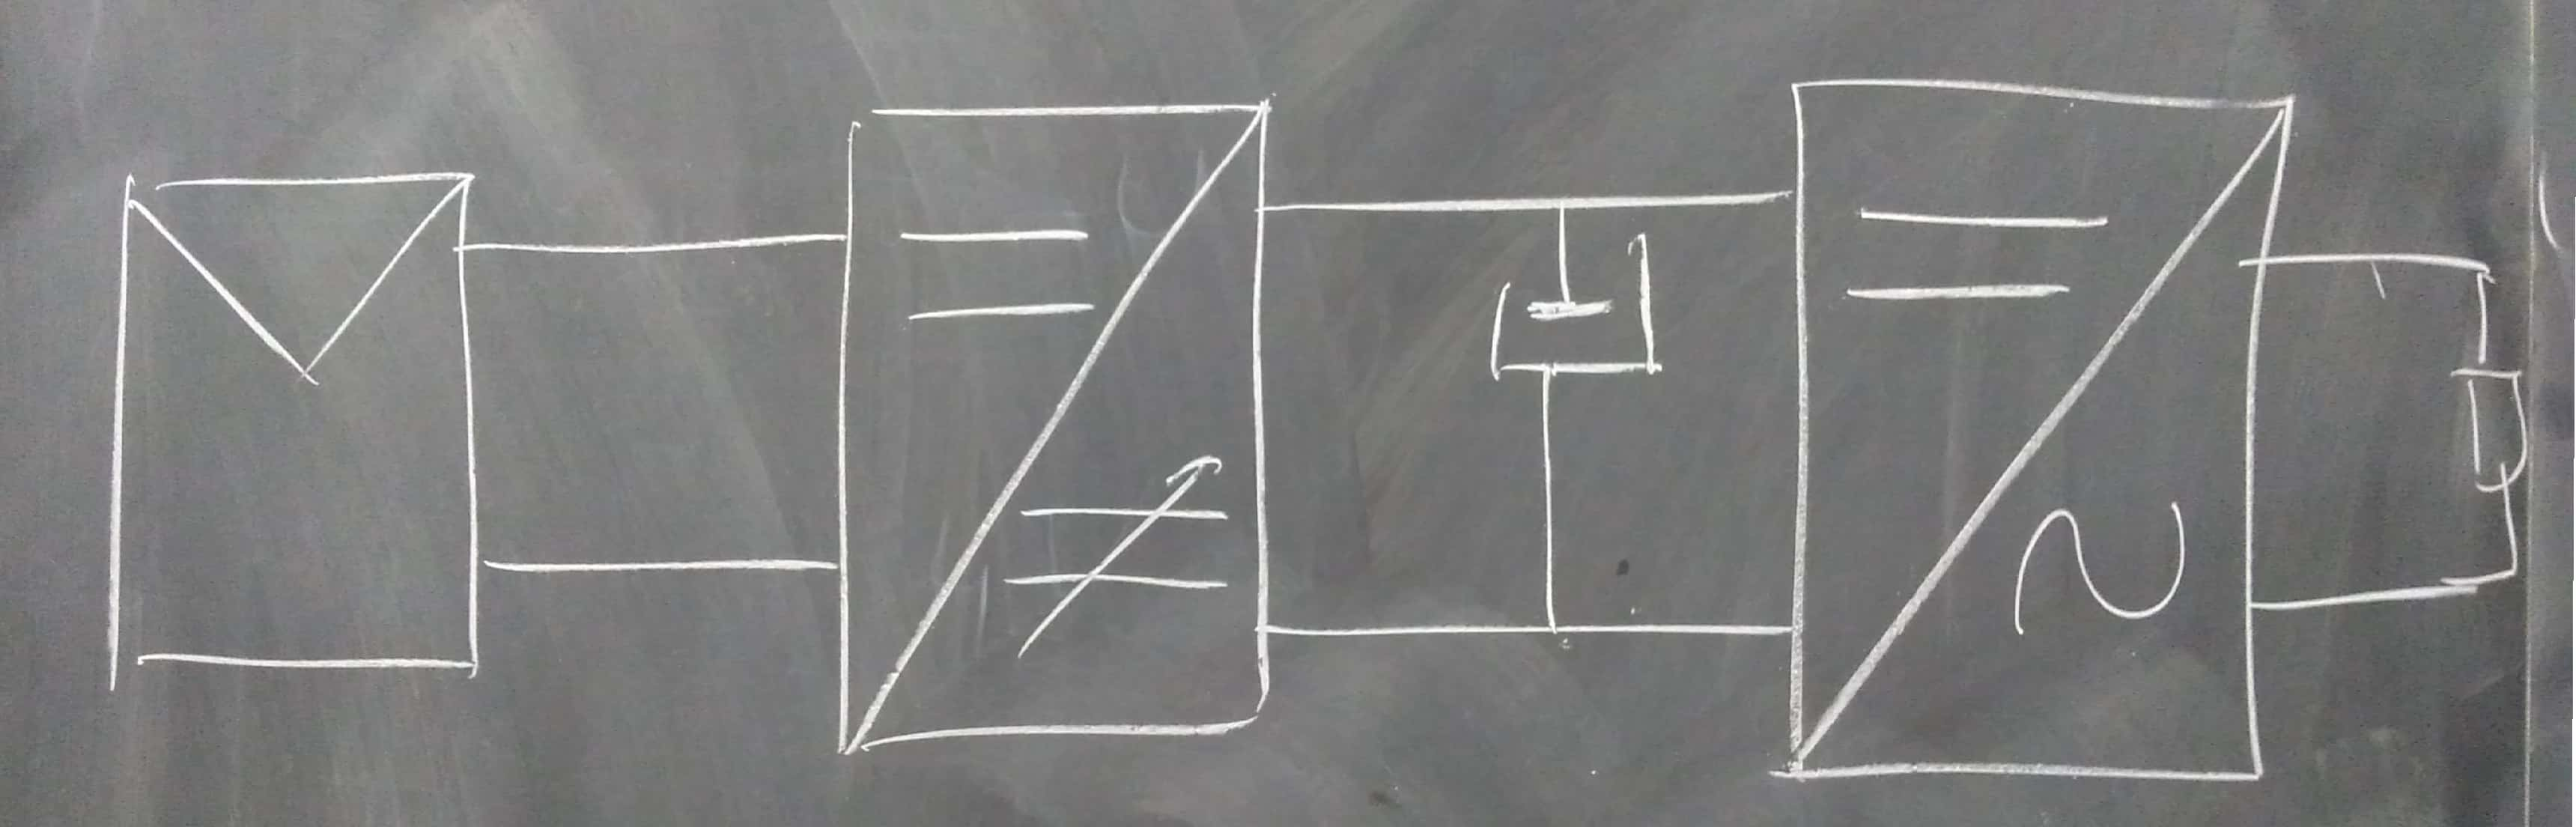
\includegraphics[width=10cm]{panneau}
\end{figure}
\centerline {panneau photovoltaïque\hspace{1.2cm}  convertisseur\hspace{1cm} onduleur \hspace{3cm}}
\section{Hacheur : convertisseur continu-continu réglable}
\begin{figure}[h]
	\centering 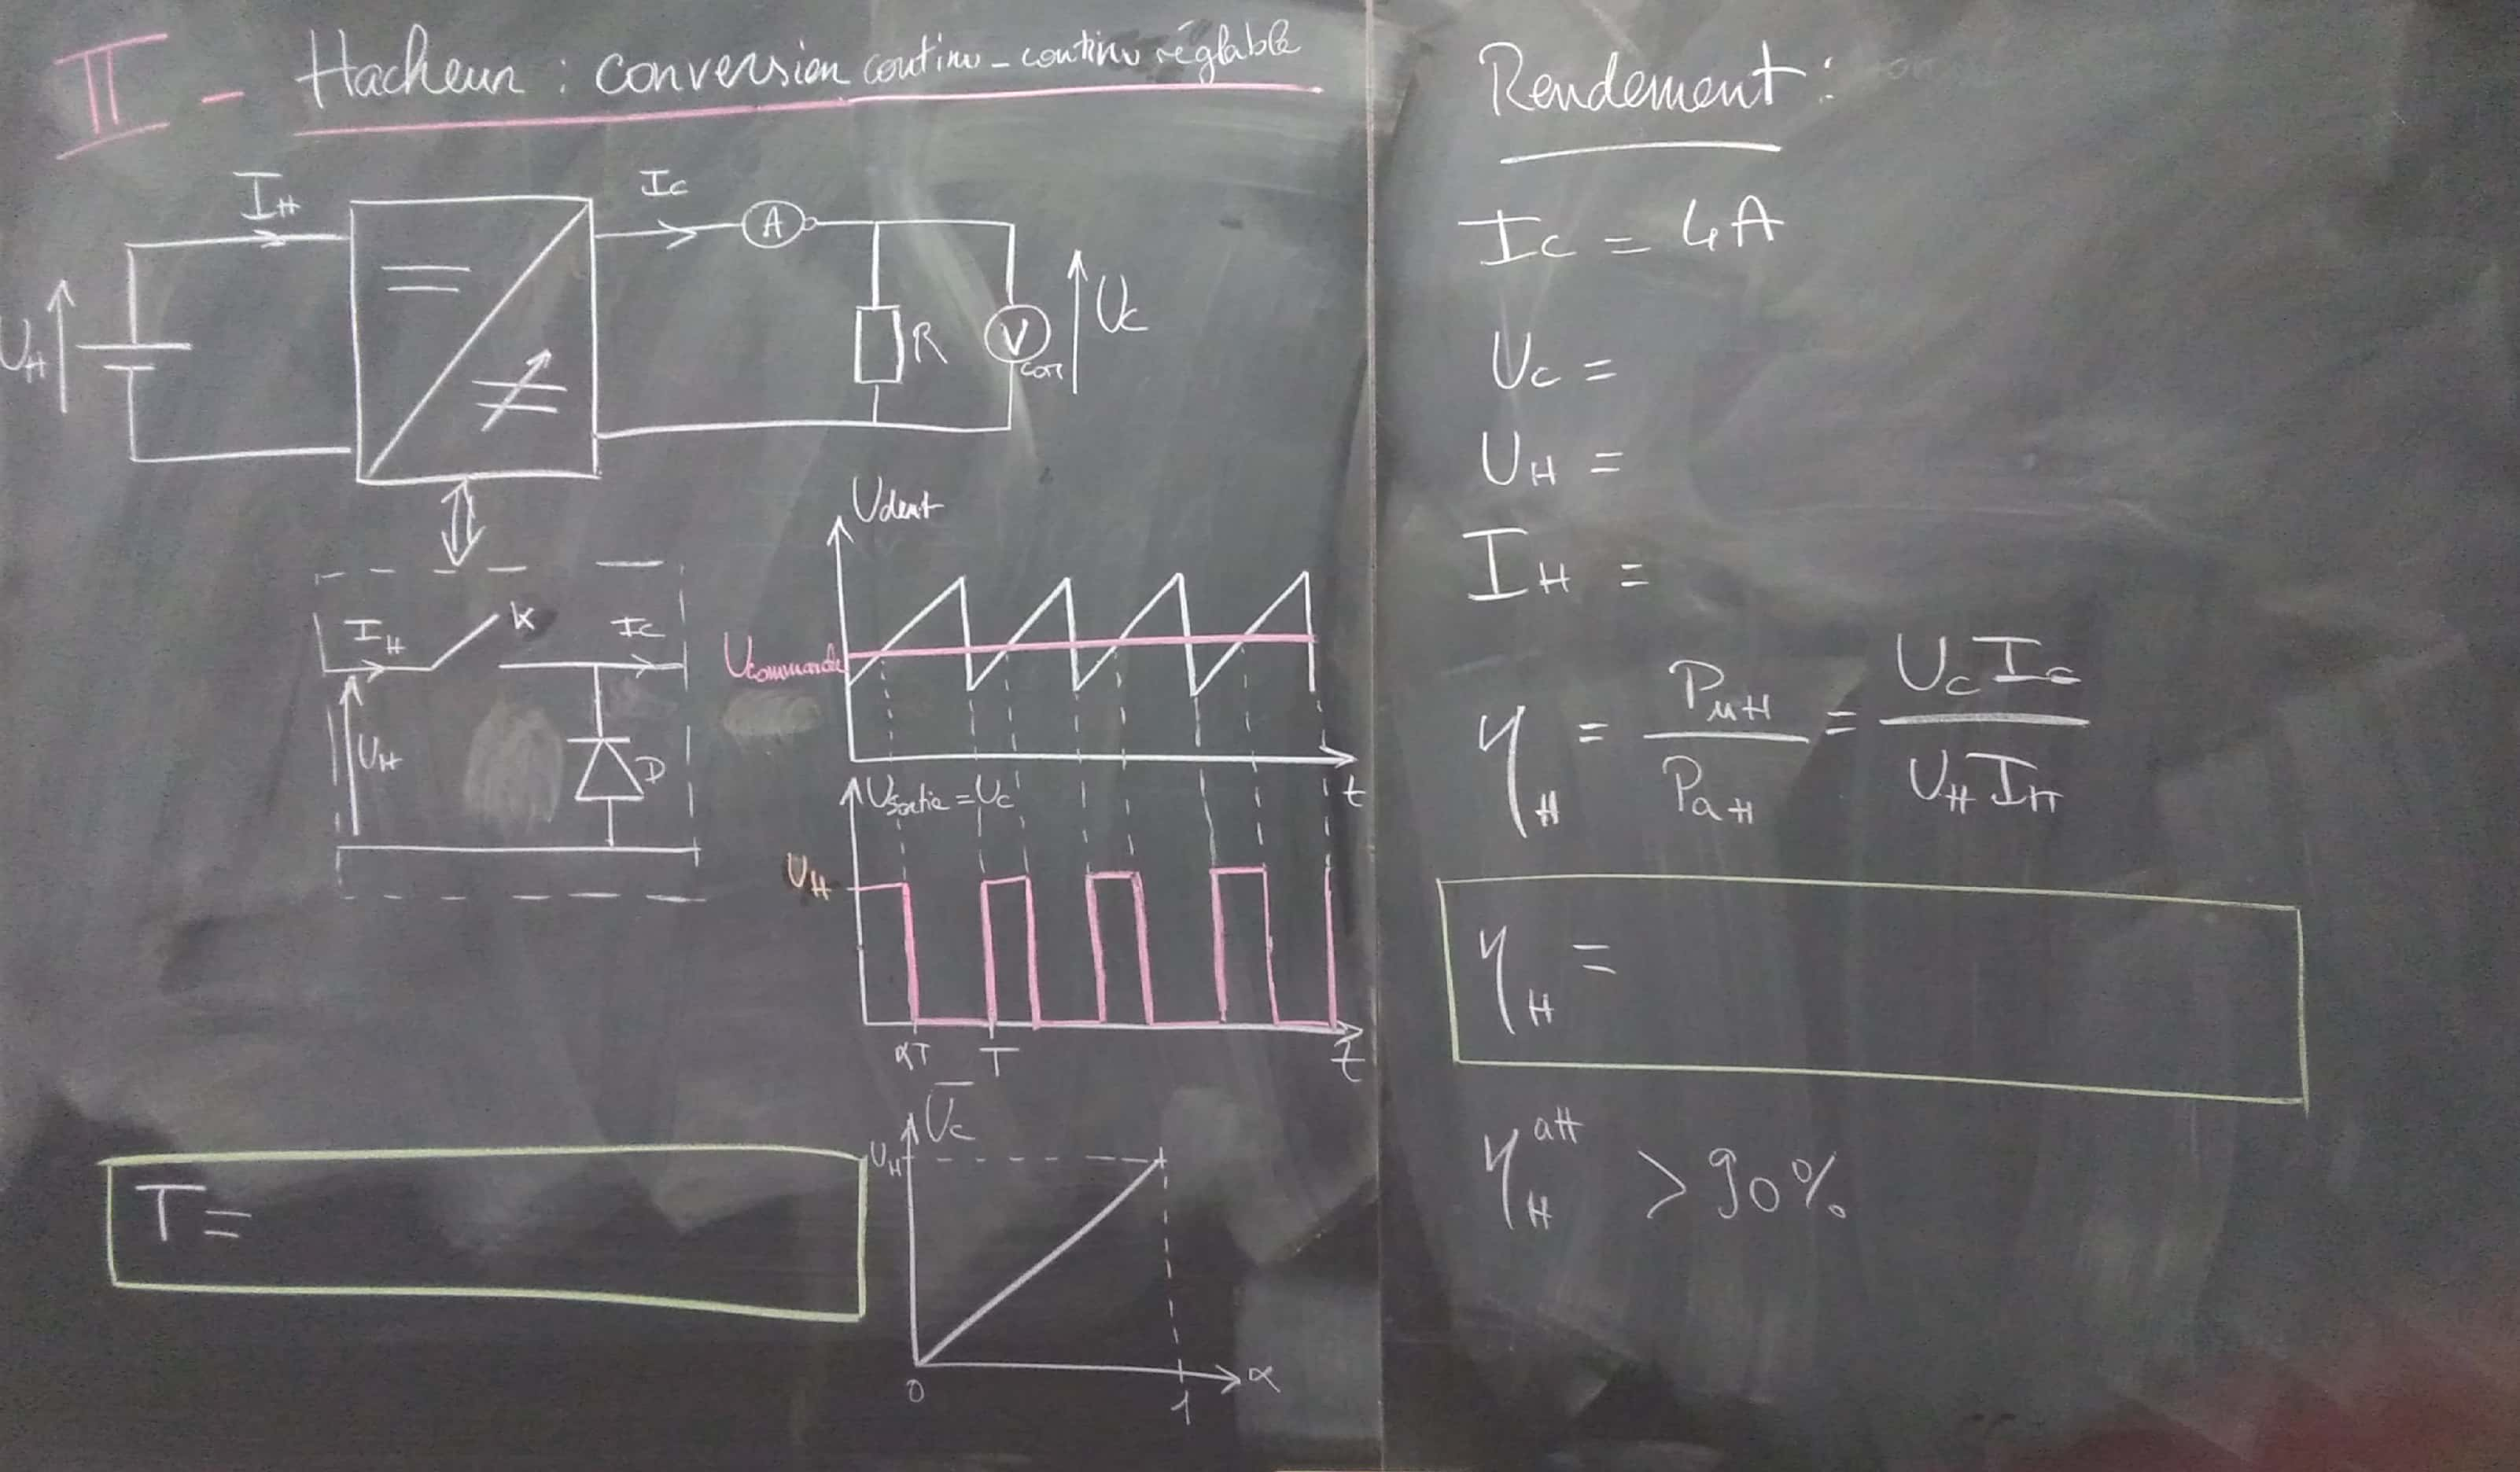
\includegraphics[width=18cm]{T2}
\end{figure}
Le hacheur est un dispositif utilisé pour modifier une tension continue, afin par exemple de modifier la vitesse de rotation d'un moteur électrique. On va en illustrer le principe ici.\\

On fait passer le courant continu produit par un générateur dans un hacheur, et on fait passer le courant dans un rhéostat sans effet inductif en sortie.\\
On commence par mesurer la période $T$, et le rapport cyclique $\alpha$ du signal généré par le hacheur. On peut ainsi vérifier que la tension de sortie $U_c$ est proportionnelle à $\alpha$.\\

On peut ensuite calculer le rendement du hacheur 
\begin{eqnarray}
\eta_H = \frac{P_{uH}}{P_{aH}} = \frac{U_cI_c}{U_HI_H}
\end{eqnarray}
à comparer avec le rendement attendu supérieur à 90\%.

\section*{Questions}
Quel sont les sources d'énergie en France ?\\
Thermonucléaire : 75\%, hydraulique : 12\%, éolien et solaire.\\

Si on double l'irradiance, que se passe t-il pour le courant ?\\
Il double.\\

Quelles sont les conditions utilisées pour les test constructeur ?\\
T = 25°C, 1000 W/h, propreté optimale... Cela explique qu'on ai pas les 5\% ici car on chauffe beaucoup le panneau.

\section*{Remarques}
alternatif à alternatif réglable : gradateur, voir schéma page suivante.

\begin{figure}[h]
	\centering 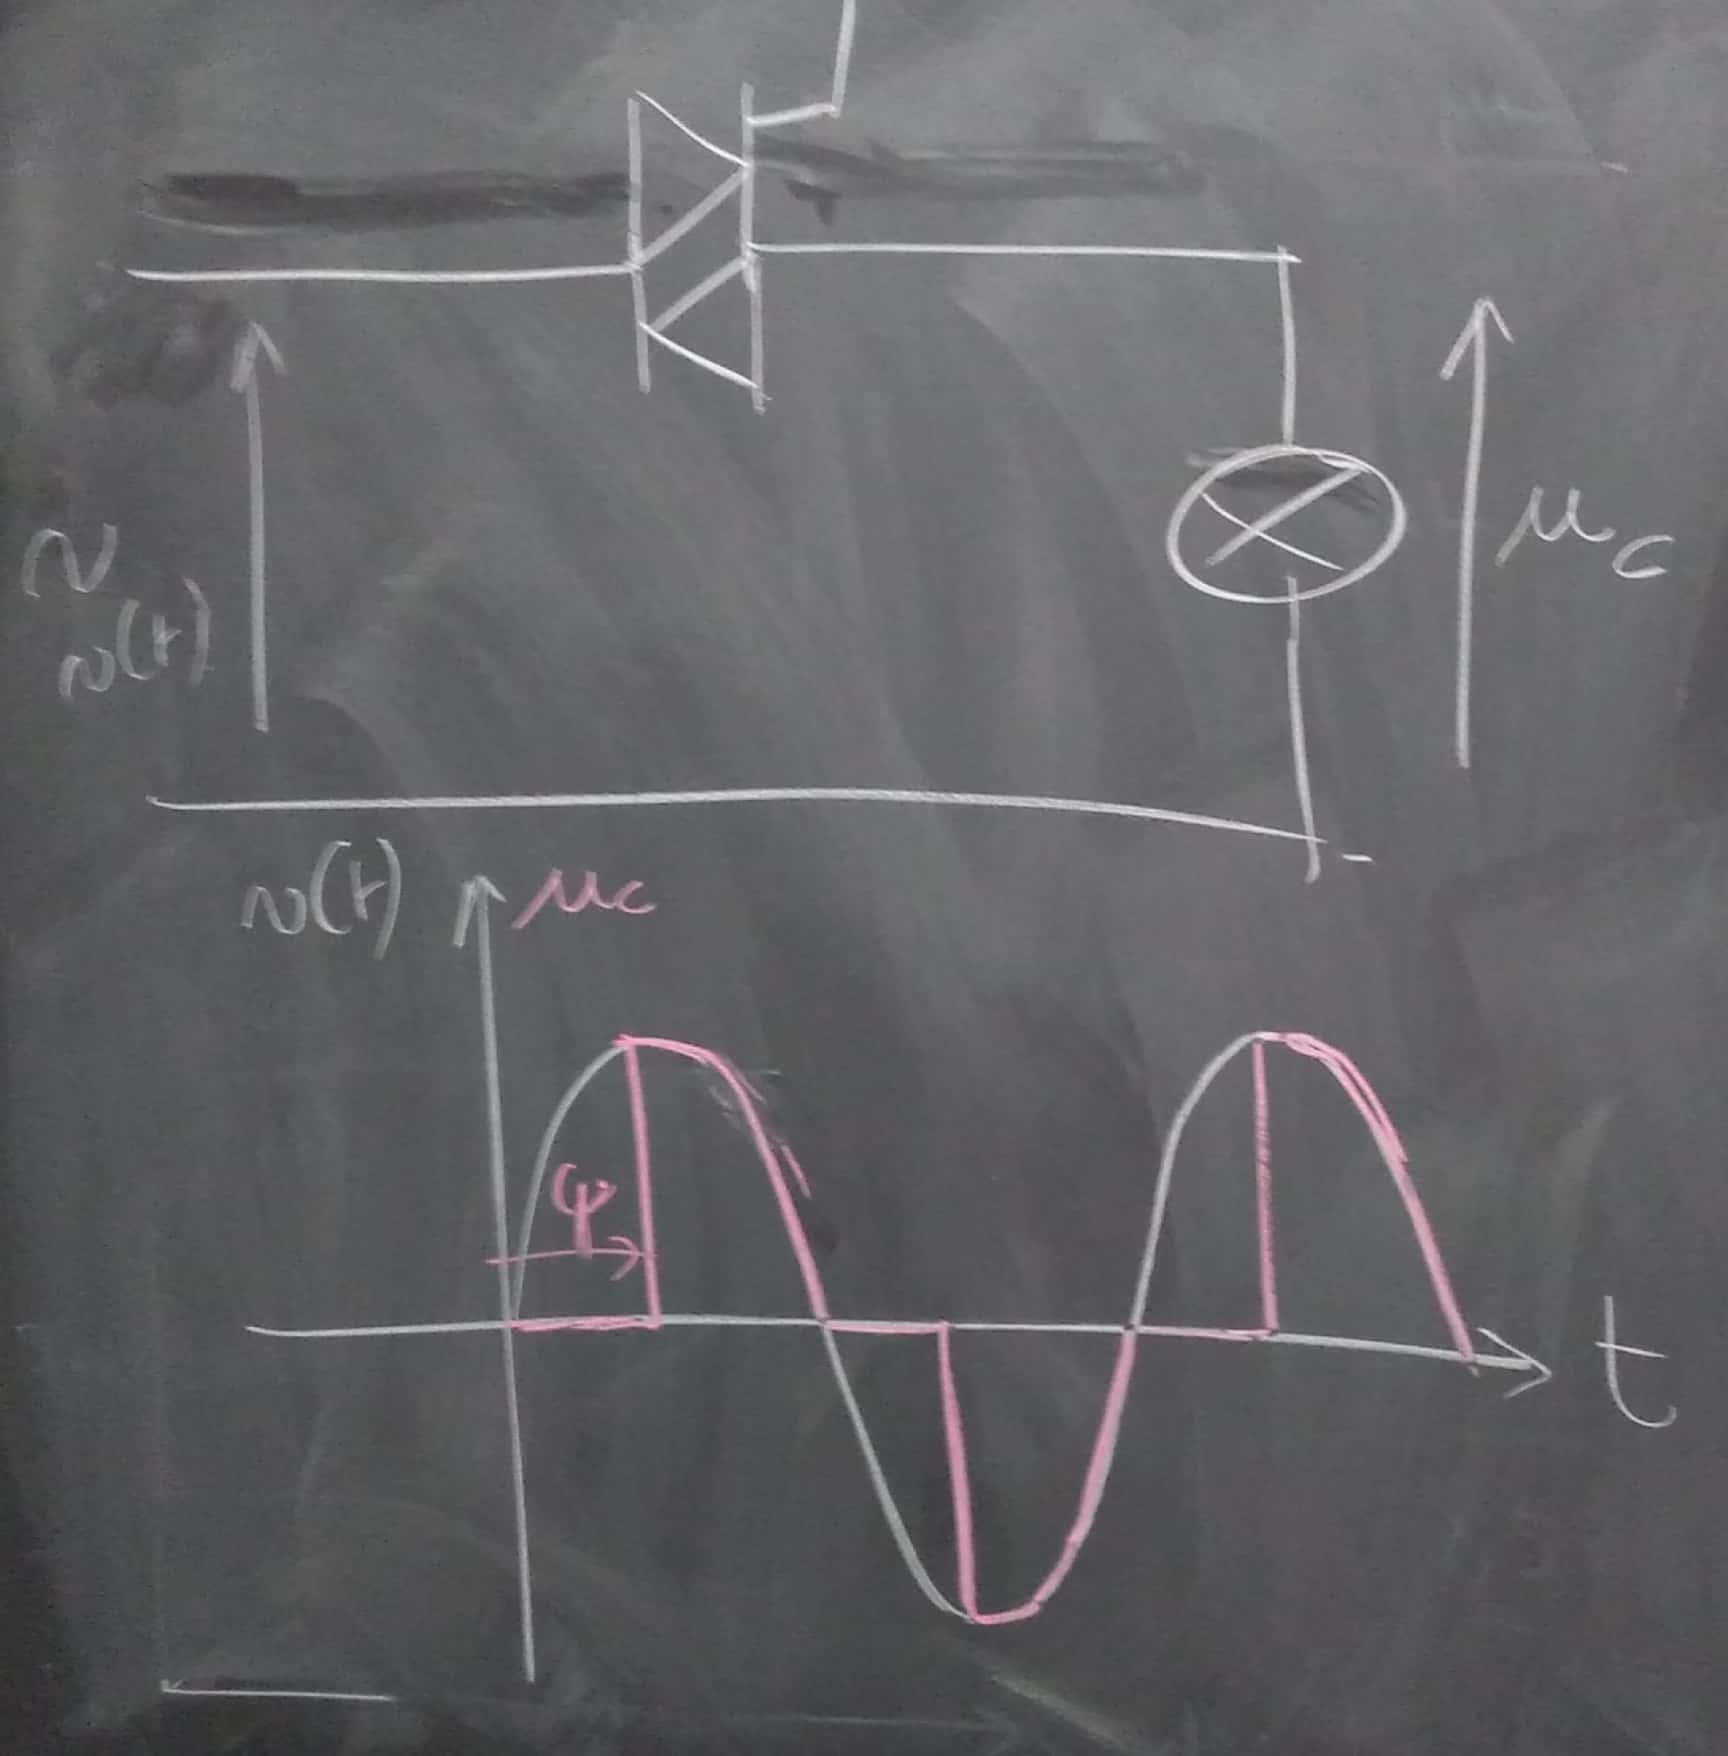
\includegraphics[width=8cm]{gradateur}
\end{figure}

\end{document}	